\chapter{Results and Discussion}
Which features contributed to classification at each level as per the EBM?

\begin{figure}[h!]
    \centering
    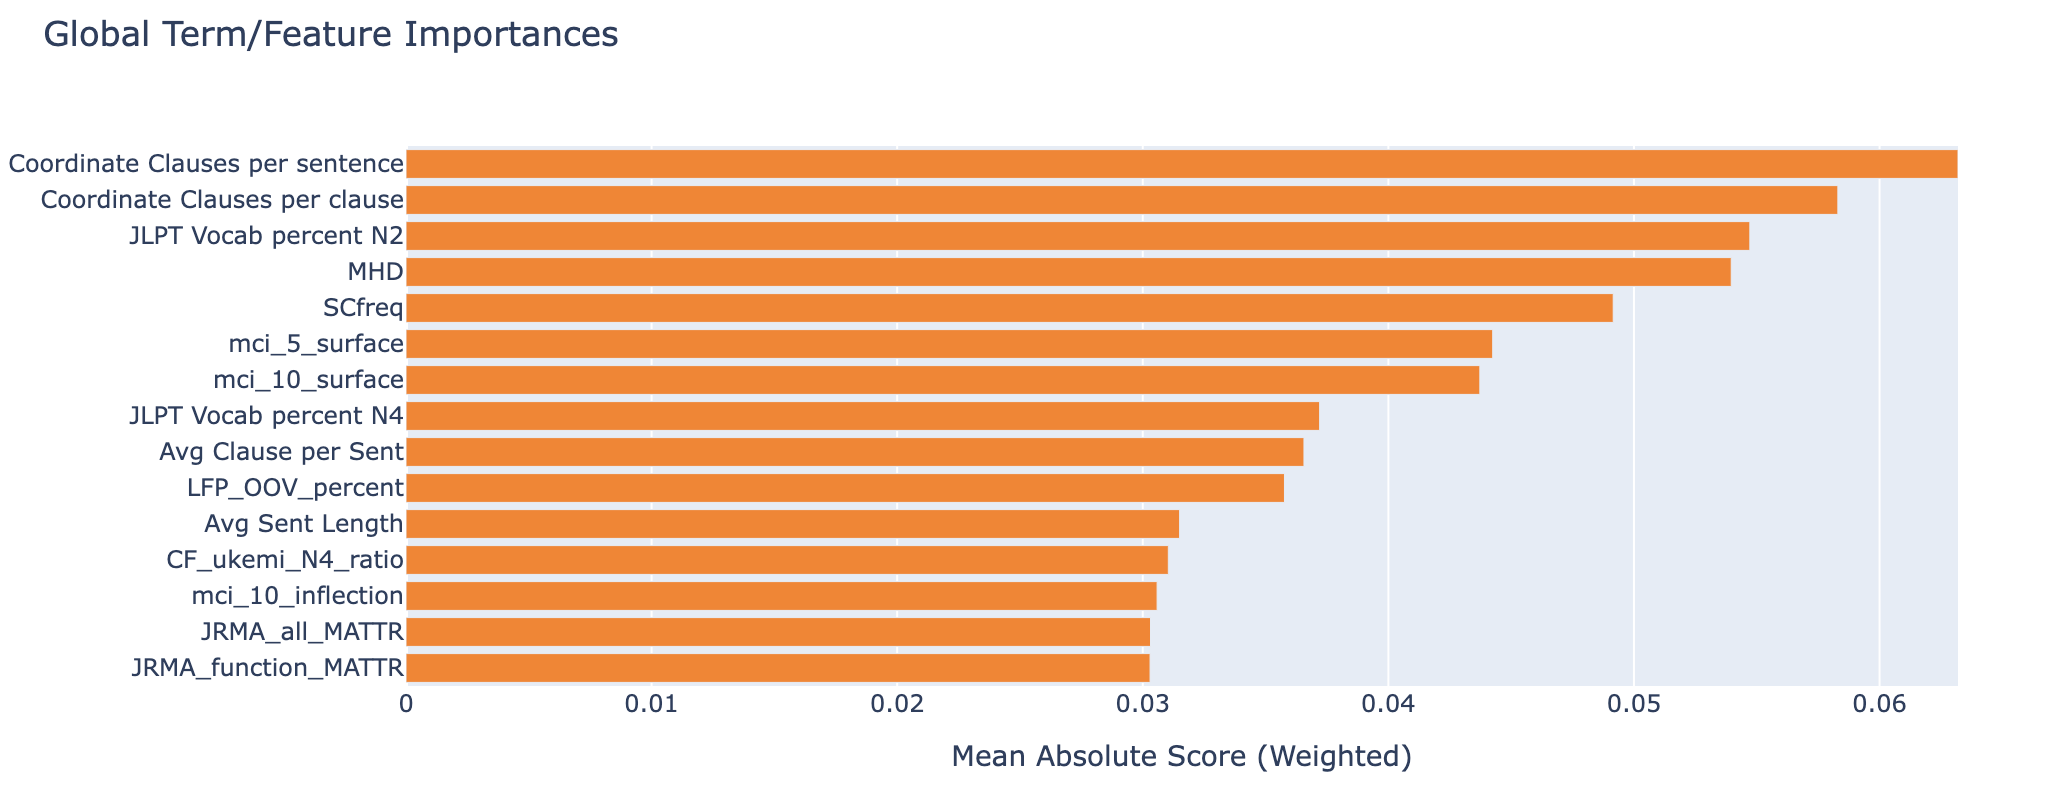
\includegraphics[scale=.4]{img/feature_importance}
    \caption{The chart of features contributing to the classificaiton of JLPT proficency levels and their weighted scores.}
    \label{fig:featureimportance}
\end{figure}

\section{Model Training Results}
*Discuss f1, accuracy, precision
*share confusion matrix
*discuss small sample size for N1 group which likely affected the classification
*could not achieve better than 50\% accuracy, probably due to the 5 groups and overlap between some proficiency
levels. Still better performance than the 20% random guess baseline....

Results:
 Overall Classification Report (All Folds Combined):
              precision    recall  f1-score   support

          N5       0.46      0.51      0.48       735
          N4       0.44      0.41      0.43      1431
          N3       0.39      0.35      0.37      1342
          N2       0.34      0.39      0.36       816
          N1       0.14      0.17      0.16       224

    accuracy                           0.39      4548
   macro avg       0.36      0.37      0.36      4548
weighted avg       0.40      0.39      0.39      4548

model had difficulty classifying N3, N2, N1 better distinguishing features needed...

\section{Discussion}
Summarize previous findings in section 4 of features and development trajectory how it aligns with the previous studies


%surprising findings:?



shortfalls/difficulties
- mention lerner language and the corpus being uncorrected so this may lead to misinterpretations by the tokenizer to classify things correctly.
    also difficulties in capturing lexical forms - many "mispellings" included on LFP OOV list.
- issue of some texts being too short for MTLD calculation
- use of only form-based grammar difficulty in correctly extracting meaning based forms
- also difficulty of not knowing which forms are considered one word expressions versus expressions that will
actually be broken down into smaller parts by the tokenizer (as noted below with 言い切る etc.) meaning not all forms
will be extracted
-small N1 group size effecting model training, and also the statistical relavance of certain features.
-Possible overlap between adjacent levels making it difficult to correctly predict....

In consistency in parsing of 〜切るto show completely finishing an action. 言い切る 売り切る are considered one verb. in the
case of 食べ(verb) 切る(非自立可能Verb) and 食べ(Verb) 切れる (AUX 非自立可能) makes it difficult to when dealing with rule based
matching to extract the form..死ぬほど and other constructions with ほどare also similar.

-Issues with clause parsing - the tokenizer by spacy is inaccurate in classyfying some coordinating and
subordinating conjunctions - many conjunctions in Japanese can be used in both contexts and spacy doesn't take the
context into consideration when labeling the conjunctions. - tried to mitigate this by using a rule based formula to
classify coordinating and subordinating clauses but it is difficult to control for each case. thereofore a more
robust system would possibly lead to better results......I need to say something more about clausal use in Japanese
for learners.


Need to mention the feature extractor follows rules for the standardized language which is widely taught to
learners. Variations due to dialects and casual written variations not included and therefore this would not be
able to extract text with these. Also chose grammar constructs which were largely form based (i.e. easier to extract
vs. use based) and ones that are likely to be used in written language. (leaving out spoken expressions as they
wouldn't likely appear much in writing. )

Mention again the shortfall of not analyzing errors or having them as a feature, this could probably lead to better
classification